\documentclass[10pt,conference,compsocconf]{IEEEtran}

\usepackage{hyperref}
\usepackage{graphicx}	% For figure environment
\usepackage{mathptmx}
\usepackage{helvet}
\usepackage{courier}
\usepackage{graphicx}
\usepackage{imakeidx} \makeindex[options = -s svind]
\usepackage{multicol}
\usepackage[bottom]{footmisc}
\usepackage{natbib}
\bibliographystyle{humannat}
\usepackage{amssymb}
\usepackage{amsmath}
\usepackage{float}
%\restylefloat{table}
%\usepackage{floatrow}
%\floatsetup[table]{capposition=top}
%\usepackage{lscape}
\usepackage{breqn}
%\usepackage{listings}
\usepackage{color}
%\usepackage[utf8]{inputenc}
%\usepackage{array}
%\definecolor{mygreen}{RGB}{28,172,0}
%\definecolor{mylilas}{RGB}{170,55,241}
\def\one{\mbox{1\hspace{-4.25pt}\fontsize{12}{14.4}\selectfont\textrm{1}}}
\newcommand{\plim}{\text{plim}}
\newcommand{\tr}{\text{tr}}
\newcommand{\diag}{\text{diag}}
\newcommand{\rank}{\text{rank}}
\newcommand{\Exp}{\text{E}}
\newcommand{\vect}{\text{vec}}
\newcommand{\vech}{\text{vech}}
\newcommand{\Var}{\text{Var}}
\newcommand{\lnf}{\text{ln f}}
\newtheorem{assumption}{Assumption}
\usepackage{amsmath}
\usepackage{breqn}
\newcommand{\R}{\mathbb{R}}

\begin{document}
\title{Project 2}

\author{
Bilguun Chinzorig, Monika Avila, Lkham Nyambuu\\
  \textit{EPFL}
}

\maketitle

\begin{abstract}
  The aim of this project is to conduct a twitter sentiment analysis. Our goal is to classify untaged tweets into two groups: positive and negative. 
  We  did a preprocessing of the tweets, generated the dictionary. We obtain the matrix of embeddings using GloVe methodology. We retrievied as feature the mean of the embeddings. Moreover, we constructed additional variables that capture the meaning  and the importance of the words as well as their importance in their part of the speech. Finally, we used our futures in two types of classifiers: 1. Random Forests (SRF) and 2. SVM. 
  We obtain that RF outperforms SVM considering both computing efficiency and classifying results. 
\end{abstract}	\textbf{ }

\section{Introduction}


In this project we perform a twitter sentiment analysis in order to classify tweets between positive and negative ones. 
For this purpose, we begin our work by preprocessing the tweets. We processed all the words in order to eliminate numbers, UrL links, duplicates and we used stems of the words. Following, we create the word space, i.e. matrix of embeddings using GloVe methodology. After, we span the tweet space by retrieving features from the embedding matrix. In addition to these features, we constructed additional variables that capture the meaning  and the importance of the words as well as hashtags included in each tweet. Finally, we used our futures in two types of classifiers: 1. Random Forests and 2. SVM. 
We conclude that random forests outperforms SVM considering both computing efficiency and classifying results. 
Random Forest achieved higher result than SVM in very low training time. And also for parameter optimization increased size of estimators in RF doesn't result over-fitting, due to it's random behavior. 
In section II we present the vocabulary construction along with the explanation of the word preprocesing. In section III we present the construction of the matrix of embeddings. Section IV explains the development of features and section V presents the models used for classification. Later, section VI describes the data used. Section VII describes the results obtaines and finally VIII draws the final conclusions. 

\section{The vocabulary construction: Word preprocesing}\label{s1}

We begin our work by preprocessing the available tweets such that we can define our vocabulary. However the words in the dataset are not easily separable by whitespaces due to following reasons:
	
	\textbf{Separators:} Words can be separated by multiple characters including whitespace for words, period for sentence ending, comma for clause endings, dash for connected words and : or ; to for beginning independent clauses. The problem is that the last two characters can be used as emojis. 

\textbf{Word contractions:} word contractions can be viewed as complete new token, but in the end it is just combination of two words. Common word contractions are related to to be's and modal verbs.

\textbf{Special words:} Due to freedom of writing tweets, we can observe multiple emphasizes on words including hashtags, and repeated characters like (hey to heyyyy). These words must have a special treatment but for vocabulary building these variations were eliminated.

\textbf{Stop words:} The full list of stop words can be found here https://kb.yoast.com/kb/list-stop-words/. In our case, we are assuming pronouns like "the" can represent some meaningful information since it emphasizes following nouns.

\textbf{Word variations:} In english word can take multiple forms like plural form, verb tenses, incorrect spelling etc. Hence, simple word separation is not enough. And also in english, people use "'s" or "s'" to represent possessions REPHRASE THIS!! 

\textbf{Numbers:} we assumed that numbers usually conveys factual informations which is not helpful to identify the opinion of a person. Moreover, we need to treat numbers different from words. Thus, we have completely removed every numbers.

In order to overcome the problems mentioned above, we created a customized vocabulary building algorithm with the following procedure:

First we tokenized the text using white space, comma, period, new line. We excluded : and ; since they are maybe part of emojis.
Following, for each token we look for word contractions. In our case, we only considered hashtags, common contraction list to separate tokens which contains multiple words. Moreover, we have removed possessions from each token.
After this, we address the issue of word variation by shrinking consecutive repeated characters, e.g. we replaced "fooooot" by "foot". Finally, we used their stems to build our vocabuary.

This preprocesing lead to an increase of the tokens in 80,000. Moreover, the total number of unique words in decreased significantly. Indeed, we have successfully obtained almost 32,000 unique words. This means that we ended up with just 32\% of all the tokens produced after splitting. (Clarify)

Now let's look at the distribution of each words. The graph \ref{fig1} shows the distribution of the words of our final vocabulary. As expected, it shows similar relationship as Zipf's law, but note that the number of words with only 1 occurence in the entire text is important. Indeed, almost 50\% of the vocabulary takes only 1.2\% of the text which implies that it is not worth keeping the 50\% of the words for simplicity.

Finally, in order to increase efficiency of the information contained in our final co-ocurence matrix we apply term frequency- inverse document frequency (tf-idf) feature. This factor gives more importance to words that are repeated in a tweet but not highly recurrent in the whole corpora.  

\begin{tiny}
		\begin{figure}[b] \label{fig1}
			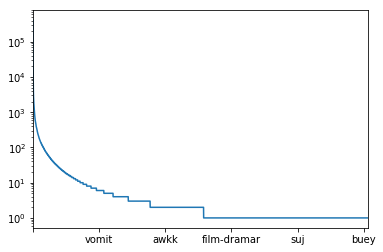
\includegraphics[scale=0.5]{WordDistribution.png}   
			\caption{Word Distribution }
			\label{fig1}    
		\end{figure}
\end{tiny}

\section{The word space: embedding matrix }\label{s2}
\label{S1}
In order to obtain a numerical representation of the words $w_i$ contained in the data set  as $\textbf{w}_{\textbf{i}} \in \mathbb{R}^K$ we used GloVE model. 

This model retrieves the numerical representation of the words that is closest to natural logarithm of the observed co-occurence value $x_{ij}$. Indeed,  \cite{pennington2014glove} propose to obtain the real valued vector by minimizing a weighted sum of squared errors. Where the error is the difference between the log of co-occurence value and the predicted one given by $\textbf{w}'_{\textbf{i}}\textbf{w}_{\textbf{j}}$. Thus, the model minimizes the following cost function: 

$$L(\textbf{w}_{\textbf{n}},\textbf{w}_{\textbf{c}})=\sum_{j=1}^{N}\sum_{i=1}^{D}f(x_{ij})(log(x_{ij})-\textbf{w}'_{\textbf{i}}\textbf{w}_{\textbf{j}})^2$$ 

with: 
$$f(x_{ij})=min(1,x_{ij}/x_{max})^{3/4}$$ 
\section{The tweet space: feature retrieval}\label{s3}
In order to obtain a numerical representation of the tweet space we can either use bag of words feature or combine individual word features appropriately.

The bag of words is a way to represent a text or sentence into vector where each feature represents one word in the vocabulary. And thus, by calculating term frequency and inverse document frequencies of each words in tweet, we can represent any given document. This method is easy to implement but needs huge amount of data in order to be effective, since number of features can be 50000 to 1 million. 

On the other hand, the most straightforward and widely used method for combining word features is taking only mean value. But two challenges of creating tweet space are loss of information related to word sequence and their emphasis. Specially most tweets has various ways of emphasizing giving word, including hash-tagging, repeating characters, emoticons etc. Hence, we also extracted the following 4 features indicating how important each word is.
\begin{enumerate}
\item Hash-tagged: boolean variable that takes value 1 if the word of tweet is hash-tagged and 0 if not. 
\item Parts of speech score: The part of speech is an important linguistic characteristic to evaluate how objective or subjective is the word. According to the (\cite{corpus}), superlatives and adjectives tend to be more subjective and thus it has more impact on evaluating writer's opinion. By using their results, we have obtained a score for each tag.
\item Negations: The negation words, including not, neither, none have important characteristics, which can completely change the meaning of the text. Thus, we created a boolean variable indicating if each word is a negation one or not. 
\item Emphasize: Many twitters use repeated characters to express their emotion. So we counted number of repeated characters in each word to represent this feature.
\end{enumerate}
Once we found the features, we combined total weight of each word feature by using following equation:


$$weight=\beta_1hash-tagged+\beta_2pos_tag+\beta_3negation+\beta_4emphasize$$

In order to find the $\beta_j$ parameters with$ j\in {1,2,3,4}$ we used grid-search algorithm which maximizes separability of negative and positive tweets' features, created from tf-idf of words.

\section{The Classification Model}\label{s4}
After obtaining the tweet space i.e. the features that represent the data set of tweets were trained in the classification model. For this aim, we used two models: 1. Random Forest and 2. SVM. 

The first model is random forests, this is a method based in an ensemble approach composed of a set of decision trees. At each node, the variables used to divide the space of the independent variables are randomly selected and used to create the decision tree (\cite{breiman2001random}). 

The second classification algorithm used is SVM. In this method, we look to maximize the geometric margin between positive and negative tweets subject to the constraint that the classified vectors must lie outside this margin\footnote{AndrewNg, Support Vector Machines}. This optimization problem is equivalent to the following one for each training sample:

$$min_w || w ||^2$$
$$s.t. \quad y_i(x'_iw +b)\geq 1$$

 Now, setting the dual problem we can obtain the support vectors which are few training observations that lie on the margin. 
 
%\section{Methods}
%\label{S2}


\section{The Data}\label{s5}
\label{S3}

Our dataset is a collection of Twitter conversations (tweets), that is divided into two different sentiments such as positive and negative messages. Each sentiments has 100000 tweets. Before the dataset analysis step, the redundant tweets needed to be deleted. We used the Notepad++ tool plugins for that purpose which gave us unique tweets. As the result, there are 91088 tweets in the negative and 90233 tweets in the positive datasets.
 
The analysis starts with comparing the usage of tags and shared links in terms of of the use of individuals either for positive or negative tweets respectively. In the graph \ref{fig2}, we can see that people use tags more than url. Furthermore, people tend to use tags more in positive massages than negative. This gives an observation that people like to share their happy moments with others by mentioning them or giving them credits. On the other hand, the usage of URL link is considerably lower than the usage of tags in the positive dataset.

\begin{tiny}
	\begin{figure}[b] \label{fig2}
		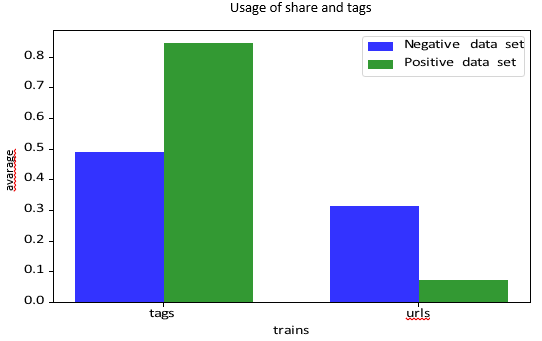
\includegraphics[scale=0.6]{Lkhamaa1.png}   
		\caption{Usage of Share and Tags }
		\label{fig2}    
	\end{figure}
\end{tiny}

After the above analysis, the links and tags needed to be deleted from the dataset because first we obtained the necessary results, and second they may be miscomputed as adjective or noun tokens. Again, we used the Notepad++ tool plugins for this purpose because it is more efficient than jupyter notebookfor computing around 90,000 tweets per dataset. Also, we had only two separate datasets so we considered the Notepad++ tool as suitable for deleting the tags and links. 

Secondly, we wanted to find out part-of-speech type of words that plays an important role in two different datasets. We counted the occurrence of every word in the datasets. In order to do that, punctuations needed to be replaced by an empty space. Also, all uppercase letters are converted into lowercase to make them identical so that they would be counted as the same word. After counting word occurrences, the words in the negative dataset are subtracted from the words used in the positive dataset. This shows the difference between the words in both datasets. 

\begin{tiny}
	\begin{figure}[b] \label{fig4}
		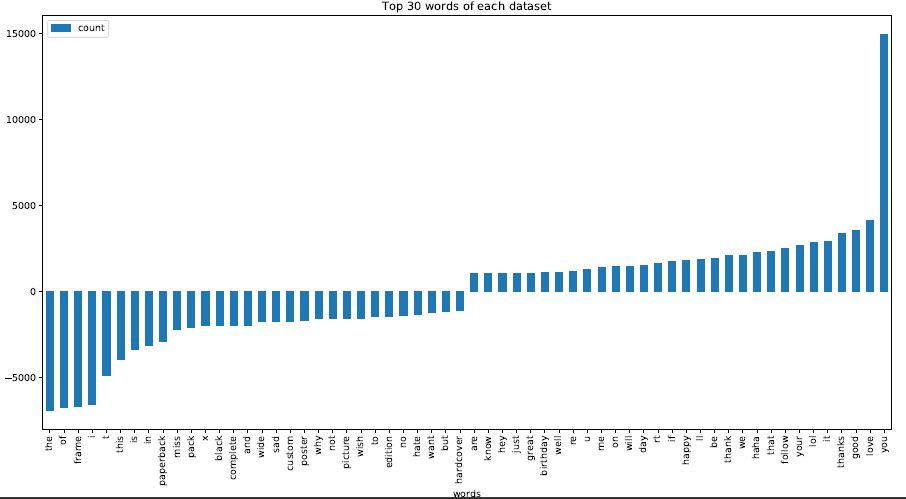
\includegraphics[scale=0.35]{Lkhamaa2.png}   
		\caption{Top 30 words of each dataset }
		\label{fig4}    
	\end{figure}
\end{tiny}

The plot \ref{fig4} shows the top 30 words of each dataset. From these 60 words, we can simply observe obvious negative and positive words respectively for each datasets. However, there are other type of words as well like prepositions and pronouns. From these words, 'You' and 'I' are very different in two datasets. 'I' is highly used in negative dataset, on the contrary, 'you' is used much more in the positive dataset. On one hand, we can conclude that people tend to blame themselves or regret for something they have done on the internet. On the other hand, the pronoun 'you' is used far more in the positive tweets, which gives a conclusion that people tend to praise or congratulate others using the Twitter. Also, the positive dataset has many retweets, which shows that people like to share positive information on the Twitter.

Adjectives play an important role in distinguishing positive and negative tweets since they are used much more, comparing to nouns and verbs, in the tweets.

After that we computed word count of each tweet starting from first to last tweet of the two datasets. We specified the words as follows.

\begin{center}
	\begin{tabular}{ |l|c|r|}
		\hline
		  & positive tweets & negative tweets \\ \hline
		min & 0 & 0 \\ \hline
		max & 46 & 37 \\ \hline
		25\% & 11.76 & 9.934 \\ \hline
		75\% & 17.23 & 14.37 \\ \hline
		mean & 17.7 & 14.54 \\ \hline
		std & 15.3 & 12.24 \\ \hline
	\end{tabular}
\end{center}



\section{Results}\label{S6}
\label{S4}
In order to analyze and evaluate our proposed pre-processing and feature processing methods, we have created 4 main pipelines.
\begin{itemize}
	\item 1. Baseline: 
	To measure impact of feature pre-processing we trained glove embeddings on raw tokens of the tweets and used RF and SVM algorithms.
	\item 2. Pre-processed:
	In this pipeline, we have used all the pre-processing methods plus word stemming to clean the data and extract words from tokens as much as possible. For word feature to tweet feature conversion, we have used the best results obtained from weighted sum method described at section 4. And finally, we trained SVM and RF algorithms to test the result.
	\item 3. Pre-trained:
	As mentioned in section 2, the vocabulary that we have extracted contains huge amount of misspelled or unrecognizable words and tokens. Thus we have used pre-trained glove word embeddings and combined them using tweet feature conversion method. And again, tested RF and SVM models.
	\item 4. Bag of words:
	After cleaning data as mentioned in section 2, we extracted tf-idf bag of words representation to describe each tweets. And used RF algorithm.
	
\begin{tiny}
	\begin{figure}[b] \label{fig5}
		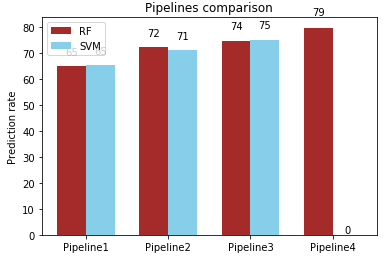
\includegraphics[scale=0.8]{results.png}   
		\caption{Results }
		\label{fig5}    
	\end{figure}
\end{tiny}

From the graph, our prediction model has increased by almost 20 percent, from 50\% to 70\%.  Also, note that even though we have lost the tweet information by generalizing the mean in pipeline 3, the result is almost same as that of RF with bag of representation. 
\end{itemize}

\section{Summary}\label{s6}
\label{S6}

Random Forest achieved higher result than SVM in very low training time. And also for parameter optimization increased size of estimators in RF doesn't result over-fitting, due to it's random behavior.
However, with both methods used we have lost word order information. This implies, there is further possibility of increasing the performance by using different model which uses sequential information, including Hidden Markov Model, Convolutional Neural Network, Ngram models etc. And moreover, according to the section 2's result many words in the vocabulary are not recognizable. Thus, there is further possibility of improvement using string matching or spell checking algorithms. But we couldn't apply them, due to computational limit. 
\bibliography{Project2}
\bibliographystyle{spbasic}
\end{document}